%
% solution.tex
%
% (c) 2021 Prof Dr Andreas Müller, OST Ostschweizer Fachhochschule
%
\documentclass[tikz]{standalone}
\usepackage{times}
\usepackage{amsmath}
\usepackage{txfonts}
\usepackage[utf8]{inputenc}
\usepackage{graphics}
\usetikzlibrary{arrows,intersections,math}
\usepackage{ifthen}
\begin{document}

\definecolor{darkgreen}{rgb}{0,0.7,0}

\newboolean{showgrid}
\setboolean{showgrid}{false}
\def\breite{7}
\def\hoehe{7}

\begin{tikzpicture}[>=latex,thick]

% Povray Bild
\node at (0,0) {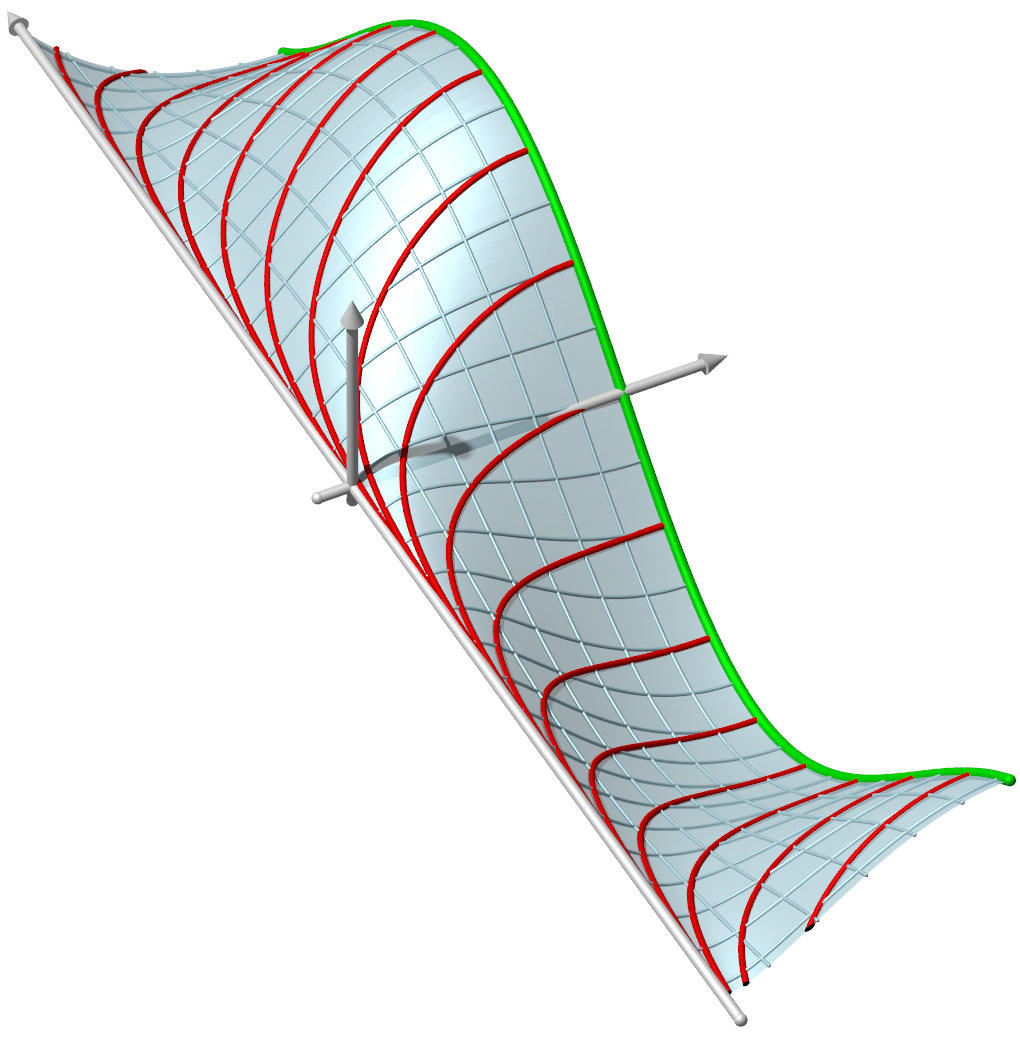
\includegraphics[width=14cm]{solution.jpg}};

% Gitter
\ifthenelse{\boolean{showgrid}}{
\draw[step=0.1,line width=0.1pt] (-\breite,-\hoehe) grid (\breite, \hoehe);
\draw[step=0.5,line width=0.4pt] (-\breite,-\hoehe) grid (\breite, \hoehe);
\draw                            (-\breite,-\hoehe) grid (\breite, \hoehe);
\fill (0,0) circle[radius=0.05];
}{}

\node at (2.8,2.5) {$x$};
\node at (-6.8,6.3) {$y$};
\node at (-1.8,2.8) {$z$};

\node[color=darkgreen] at (0,6) [right] {$u(\frac{\pi}2,y_0)=\sin(y_0)$};

\end{tikzpicture}

\end{document}

